\documentclass[12pt, a4paper, oneside]{ctexart}
\usepackage{amsmath, amsthm, amssymb, appendix, bm, graphicx, hyperref, mathrsfs}
\usepackage{fontspec}
\usepackage{listings}
\usepackage{color}
\usepackage{xcolor}
\definecolor{dkgreen}{rgb}{0,0.6,0}
\definecolor{gray}{rgb}{0.5,0.5,0.5}
\definecolor{mauve}{rgb}{0.58,0,0.82}
\lstset{frame=tb,
     language=Java,
     aboveskip=3mm,
     belowskip=3mm,
     showstringspaces=false,
     columns=flexible,
     basicstyle = \ttfamily\small,
     numbers=left,
     numberstyle=\tiny\color{gray},
     keywordstyle=\color{blue},
     commentstyle=\color{dkgreen},
     stringstyle=\color{mauve},
     breaklines=true,
     breakatwhitespace=true,
     tabsize=4
}

\CTEXsetup[format={\Large\bfseries}]{section}

\title{\textbf{测试计划}}
\author{第25组}
\date{\today}

\begin{document}


\maketitle
\section{概述}
\subsection{测试需求}
本次作业要求使用白盒测试。我们选择了一个红黑树的java实现作为测试对象,使用Junit框架进行单元测试。

\subsection{任务分配}
本小组为四人小组,任务分配为:

\subsection{总体思路}
由于被测软件有很多方法是private的方法,\textbf{为了使得测试方便,我们将所有方法全部改成public}。原软件的所有public接口,写在RBTree.java顶部的注释中。

首先, colorOf 和 parentOf 等简单的accessor方法,以及 setColor 等简单的set方法,可以看做类似于宏,不需要进行单元测试,\textbf{只要其他方法的单元测试通过了,这些方法必然被覆盖到}。

因此,先测试各个查找方法。然后在测试修改树结构有关的方法时,首先需要测试左旋、右旋方法,然后测试重新平衡方法。最后再测试插入、删除方法。在本测试计划中,以下各个的单元测试是按照顺序进行的。


\section{对search方法的测试}

search方法代码如下。在实际使用中,search一定是从根节点开始查找,因此两个方法可以合并测试。

\begin{lstlisting} [language = Java]
public RBTNode<T> search(RBTNode<T> x, T key) {
    if (x==null)
        return x;

    int cmp = key.compareTo(x.key);
    if (cmp < 0)
        return search(x.left, key);
    else if (cmp > 0)
        return search(x.right, key);
    else
        return x;
}

public RBTNode<T> search(T key) {
    return search(mRoot, key);
}
\end{lstlisting}

\subsection{DD路径分析和数据流分析}

各个节点的定义如下

\newpage
\begin{table}[!h]
    \begin{tabular}{|l|l|}
    \hline
    代码行 & DD路径名称\\ \hline
    1 & A\\ \hline
    2 & B\\ \hline
    3 & C \\ \hline
    5 & D \\ \hline
    6 & E \\ \hline
    7 & F \\ \hline
    8 & G \\ \hline
    9 & H \\ \hline
    10-11 & I \\ \hline
    12 & J \\ \hline
    12-end & K \\ \hline
    \end{tabular}
\end{table}

其中,12-end描述的行为是在接收函数返回值并退出。


递归是一种特殊的循环。因此可以分析DD路径如下

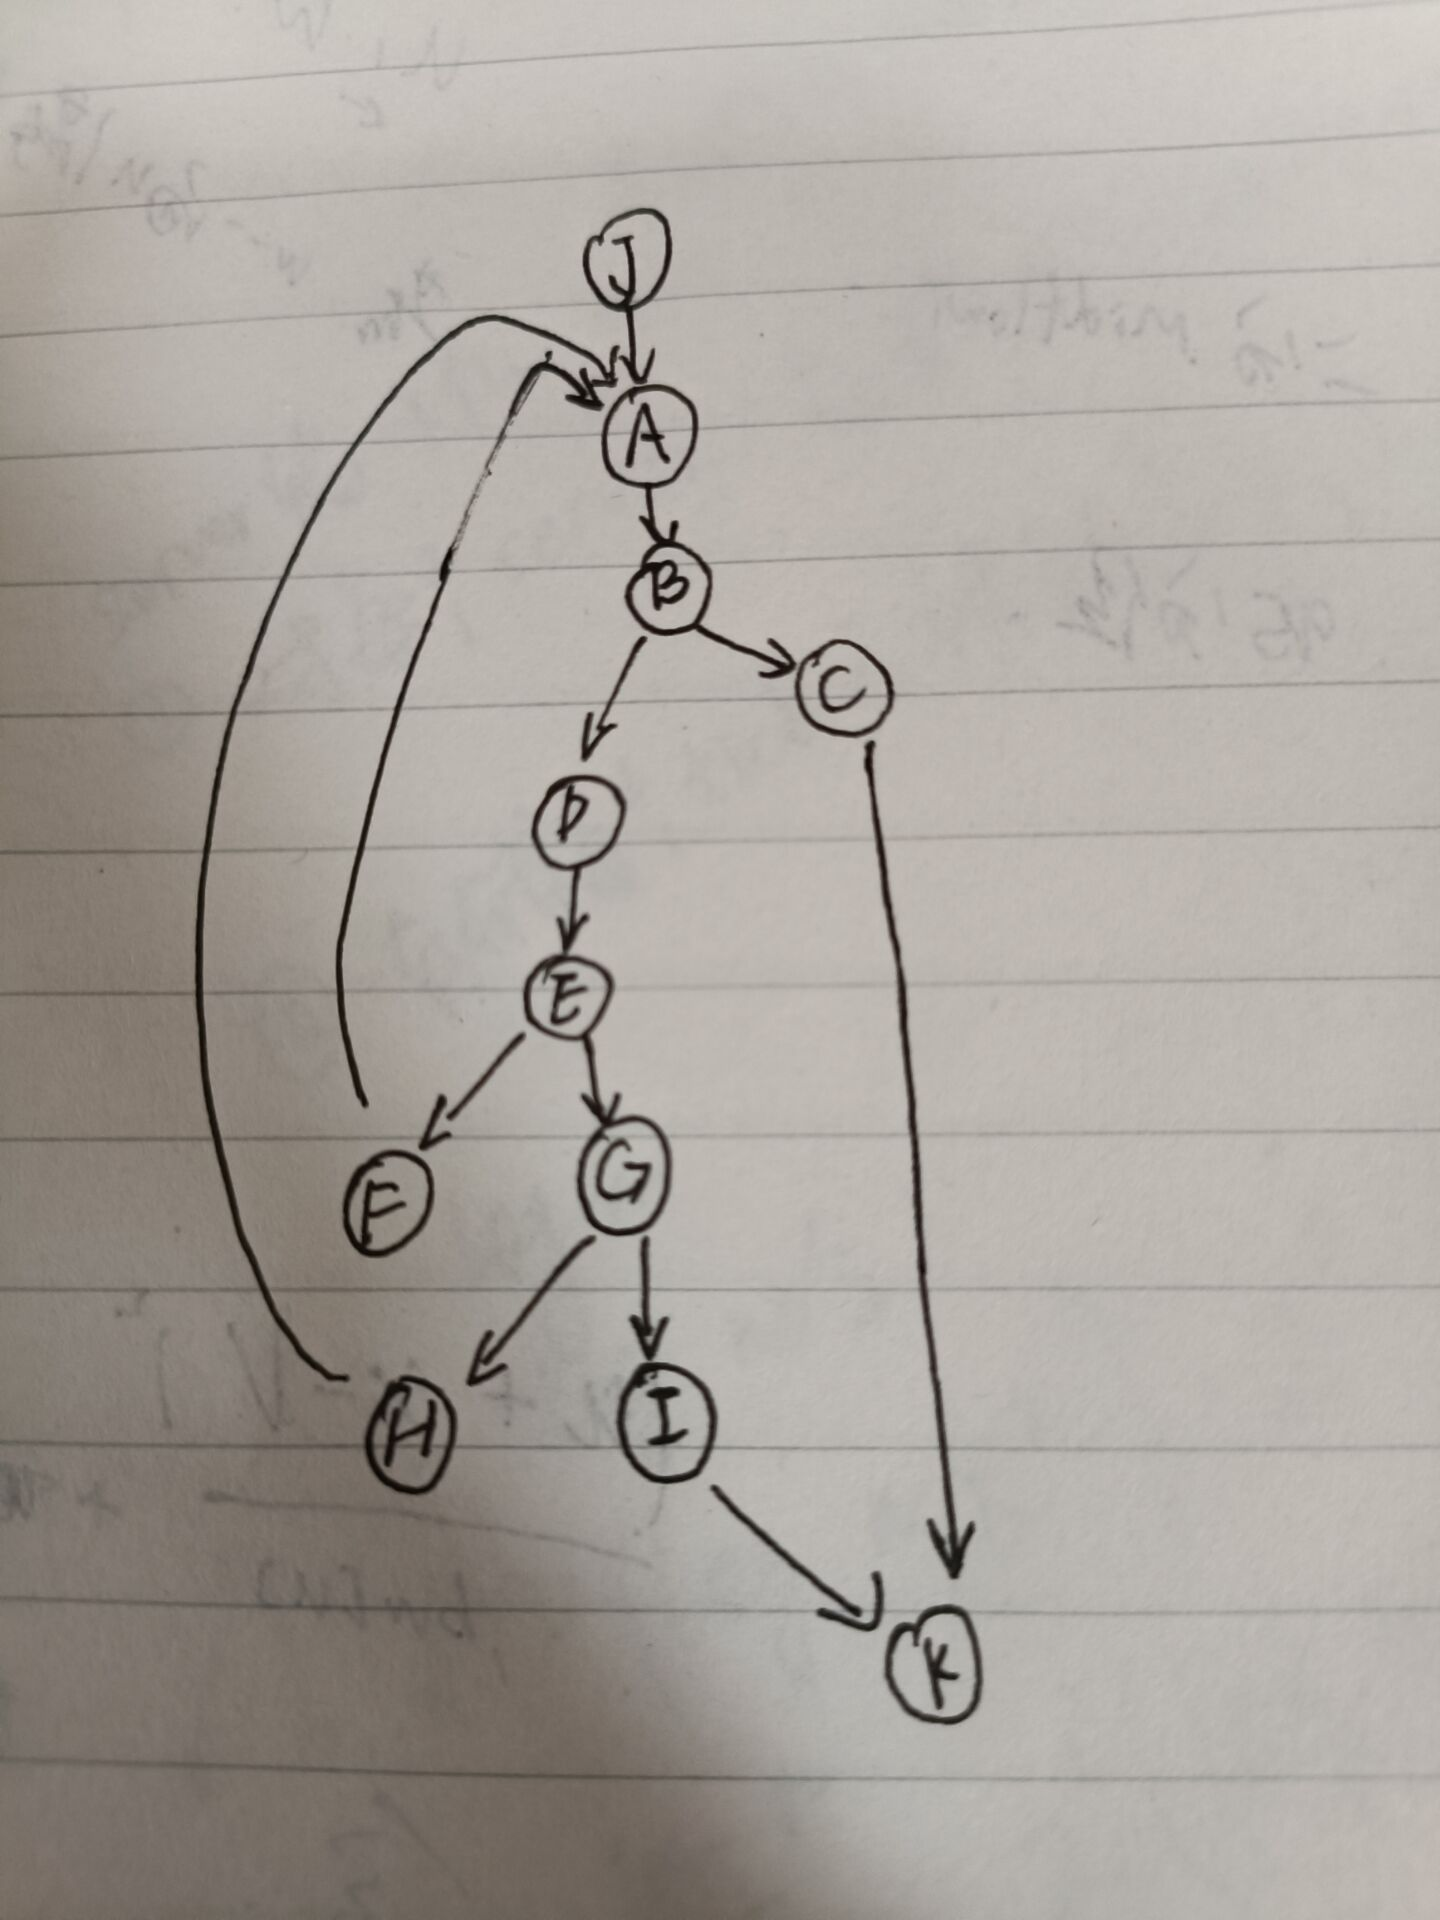
\includegraphics[scale=0.2]{screenshots/DD-search.jpg}

数据流分析如下

\begin{table}[!h]
    \begin{tabular}{|l|l|l|}
    \hline
    变量名 & 定义节点 & 使用节点 \\ \hline
    x & A & B C D F H I\\ \hline
    key & A & F H \\ \hline
    cmp & D & E G \\ \hline
    \end{tabular}
\end{table}

在这个方法的单元测试中,使用数据流分析的结果设计用例,覆盖指标采用\textbf{全使用准则}。
因此,测试用例的执行路径集合,需要覆盖以下路径:A-B, A-C, A-D, A-F, A-H, A-I, D-E, D-G.

\subsection{用例设计}

首先构造一个红黑树,然后依次查询权值为5, 6, 114514的节点。红黑树的形态如下图所示:

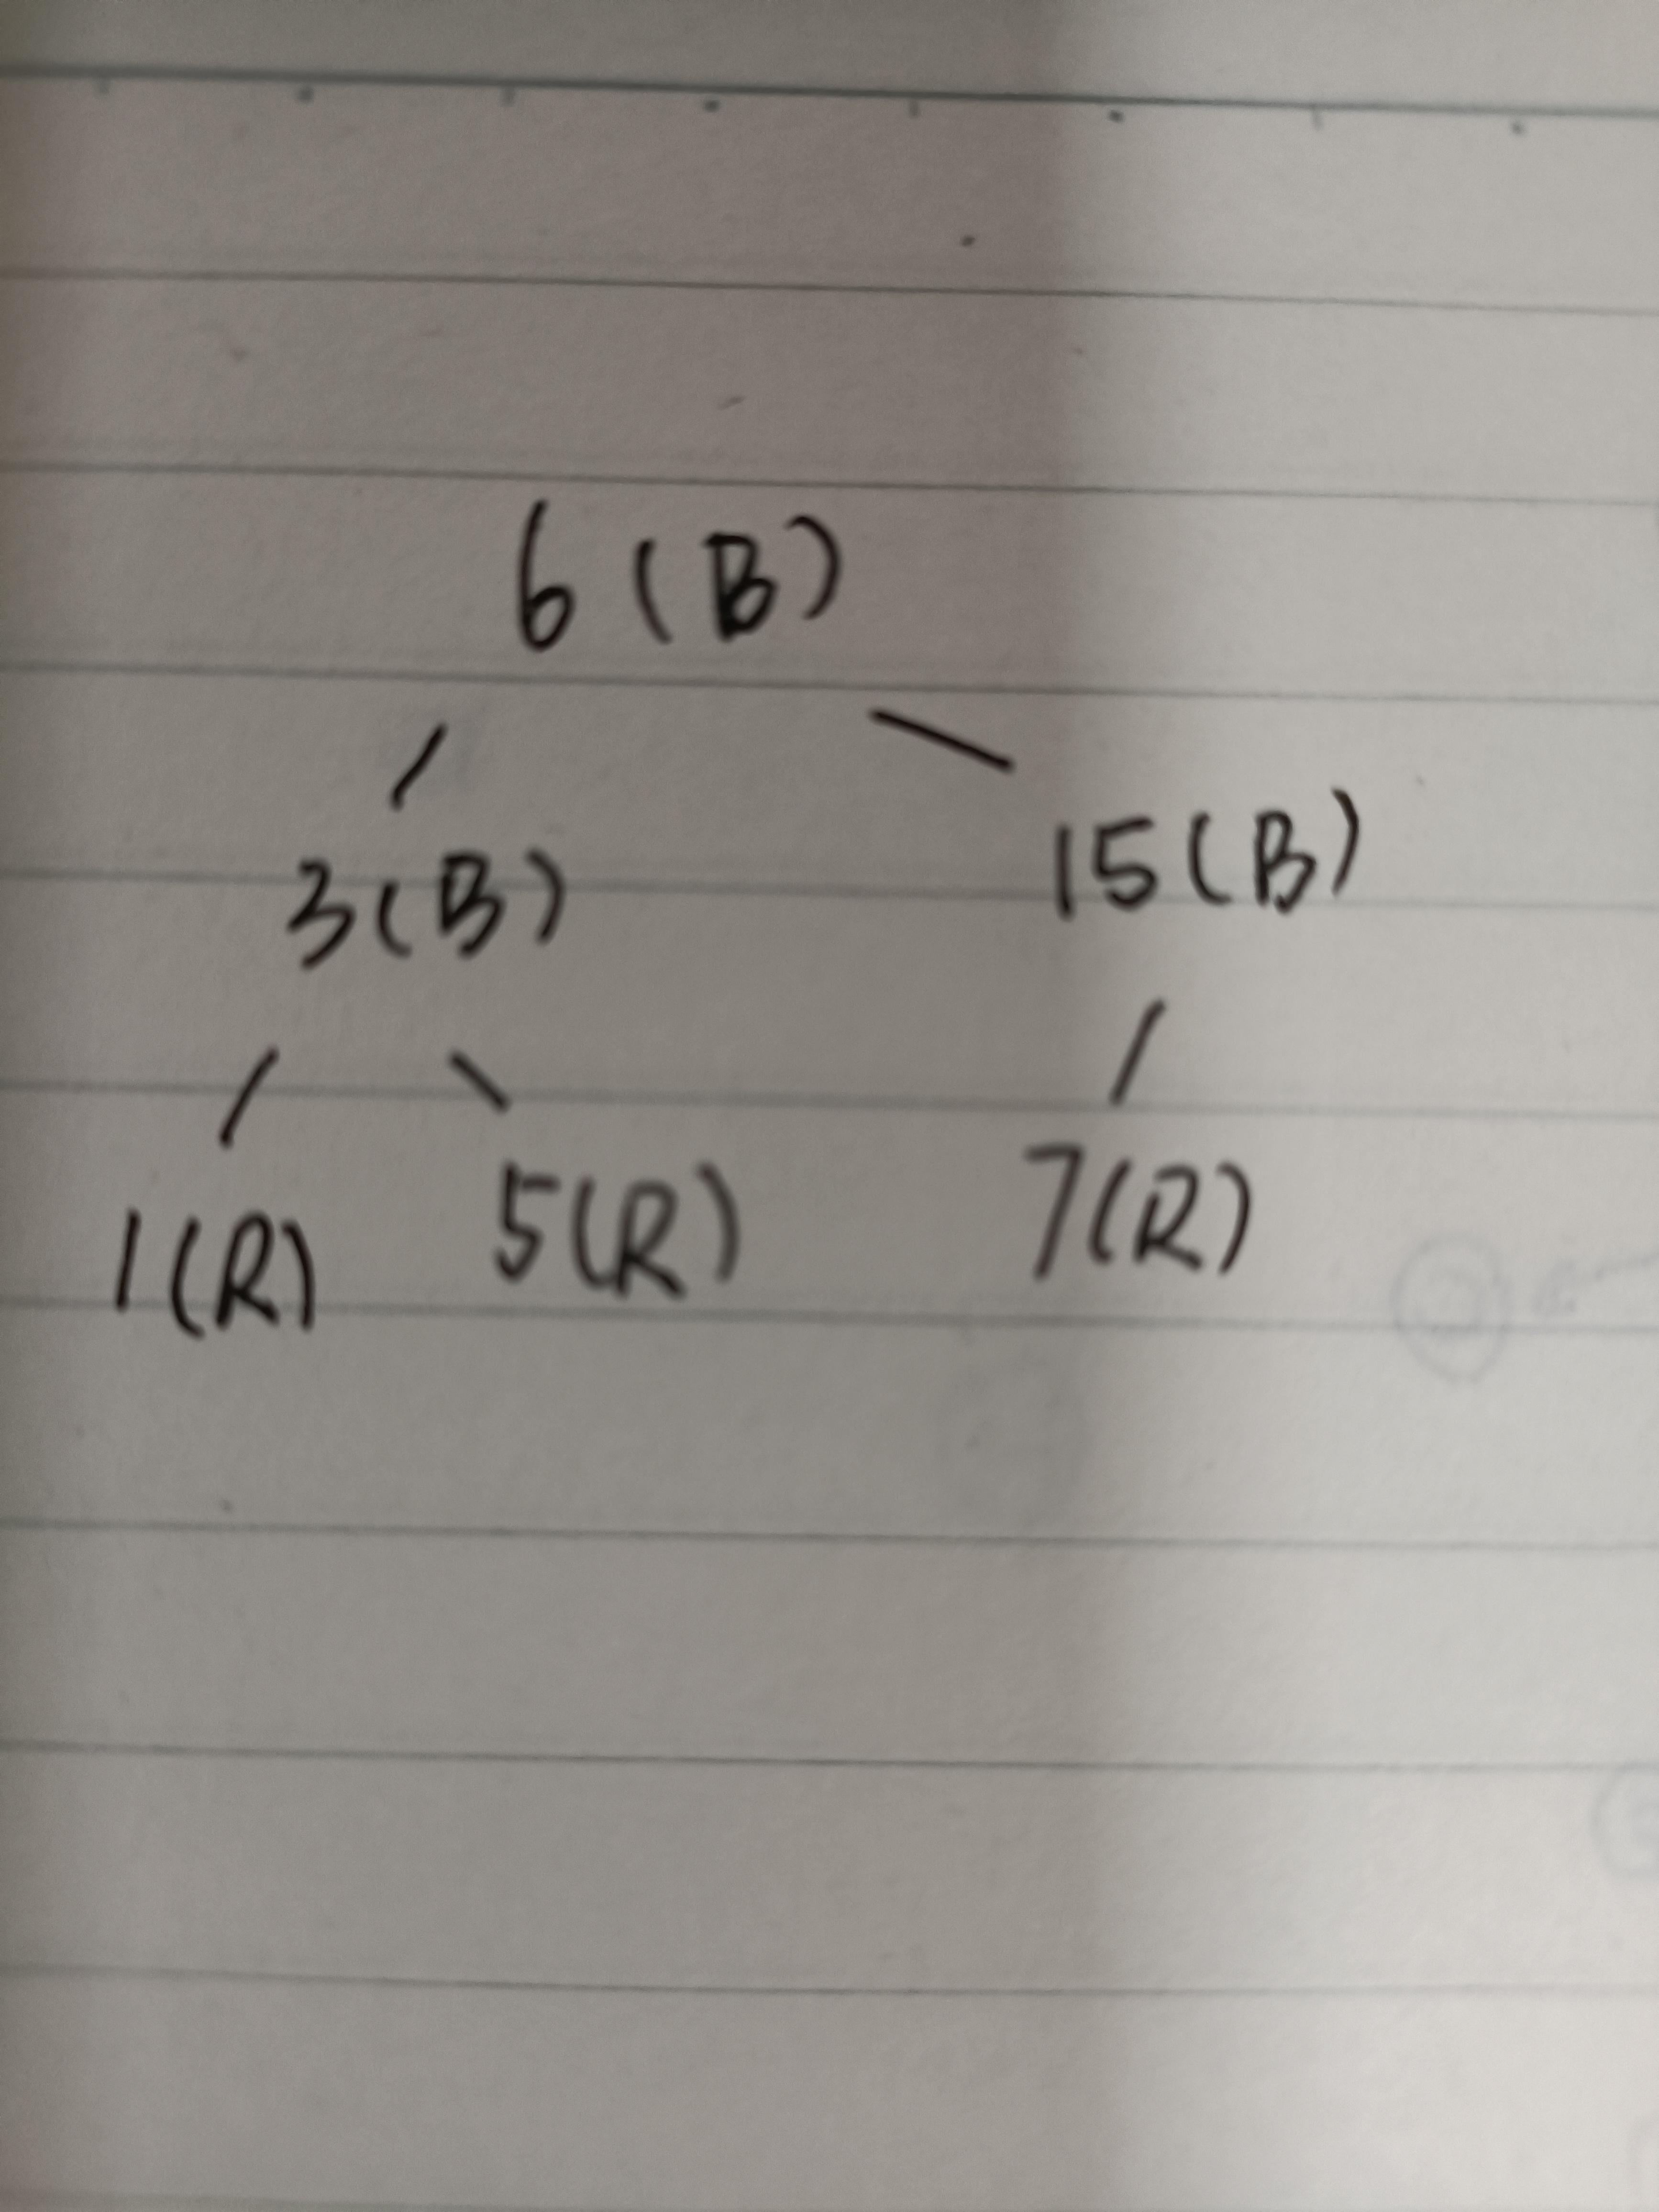
\includegraphics[scale=0.07]{screenshots/RBT-search.jpg}

具体可见代码实现。

\section{对minimum方法的测试}

minimum方法代码如下。

\begin{lstlisting} [language = Java]
public T minimum() {
    if (mRoot == null)
        return null;

    RBTNode<T> p = mRoot;
    while (p.left != null)
        p = p.left;

    return p.key;
}
\end{lstlisting}

\subsection{DD路径分析和数据流分析}

各个节点的定义如下

\begin{table}[!h]
    \begin{tabular}{|l|l|}
    \hline
    代码行 & DD路径名称\\ \hline
    1 & A\\ \hline
    2 & B\\ \hline
    3 & C \\ \hline
    5 & D \\ \hline
    6 & E \\ \hline
    7 & F \\ \hline
    9 & G \\ \hline
    \end{tabular}
\end{table}

DD路径如下

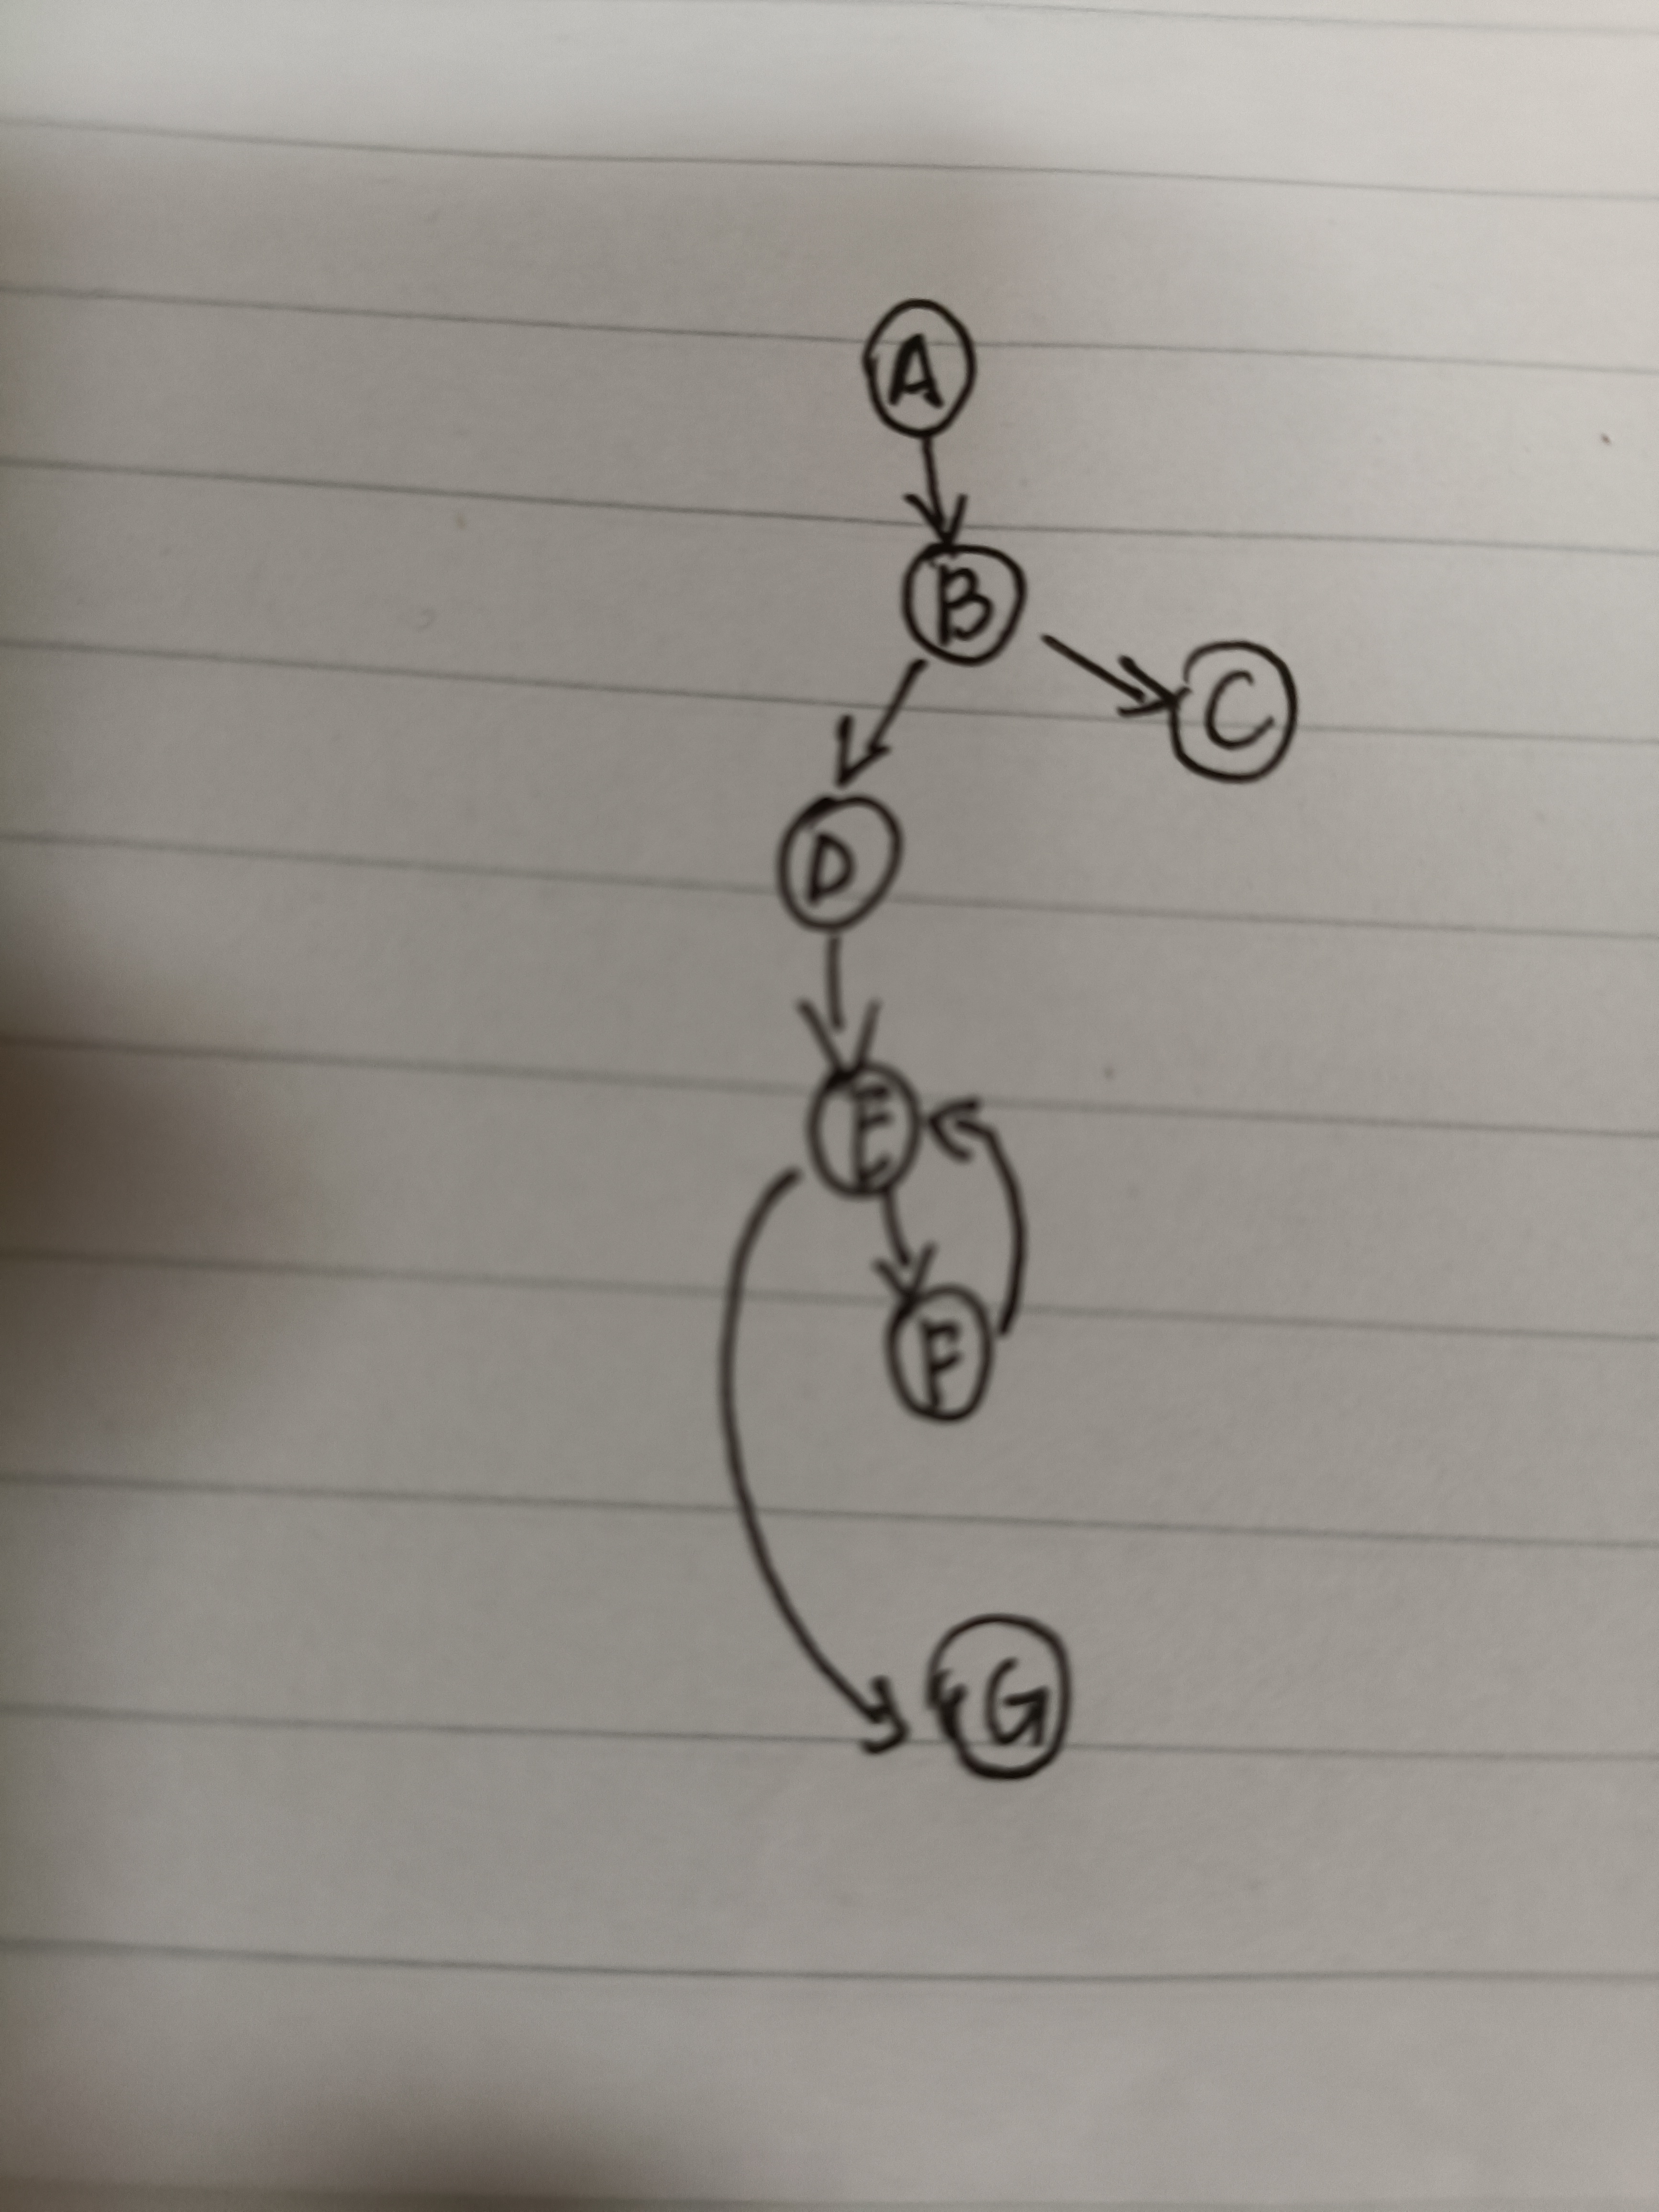
\includegraphics[scale=0.06]{screenshots/DD-minimum.jpg}

数据流分析如下

\begin{table}[!h]
    \begin{tabular}{|l|l|l|}
    \hline
    变量名 & 定义节点 & 使用节点 \\ \hline
    this.mRoot & A & B D\\ \hline
    p & D & E F G \\ \hline
    \end{tabular}
\end{table}

在这个方法的单元测试中,使用数据流分析的结果设计用例,覆盖指标采用\textbf{全使用准则}。
因此,测试用例的执行路径集合,需要覆盖以下路径:A-B, A-D, D-E, D-F, D-G.

\subsection{用例设计}

在红黑树为空的时候,查询一次minimum。然后构建一棵与search方法单元测试中相同的红黑树,再查询一次minimum。具体可见代码实现。

\section{对maximum方法的测试}

maximum方法与minimum方法几乎一致,代码如下

\begin{lstlisting} [language = Java]
public T maximum() {
    if (mRoot == null)
        return null;

    RBTNode<T> p = mRoot;
    while (p.right != null)
        p = p.right;

    return p.key;
}
\end{lstlisting}

\subsection{DD路径分析和数据流分析}

各个节点的定义如下

\begin{table}[!h]
    \begin{tabular}{|l|l|}
    \hline
    代码行 & DD路径名称\\ \hline
    1 & A\\ \hline
    2 & B\\ \hline
    3 & C \\ \hline
    5 & D \\ \hline
    6 & E \\ \hline
    7 & F \\ \hline
    9 & G \\ \hline
    \end{tabular}
\end{table}

DD路径如下

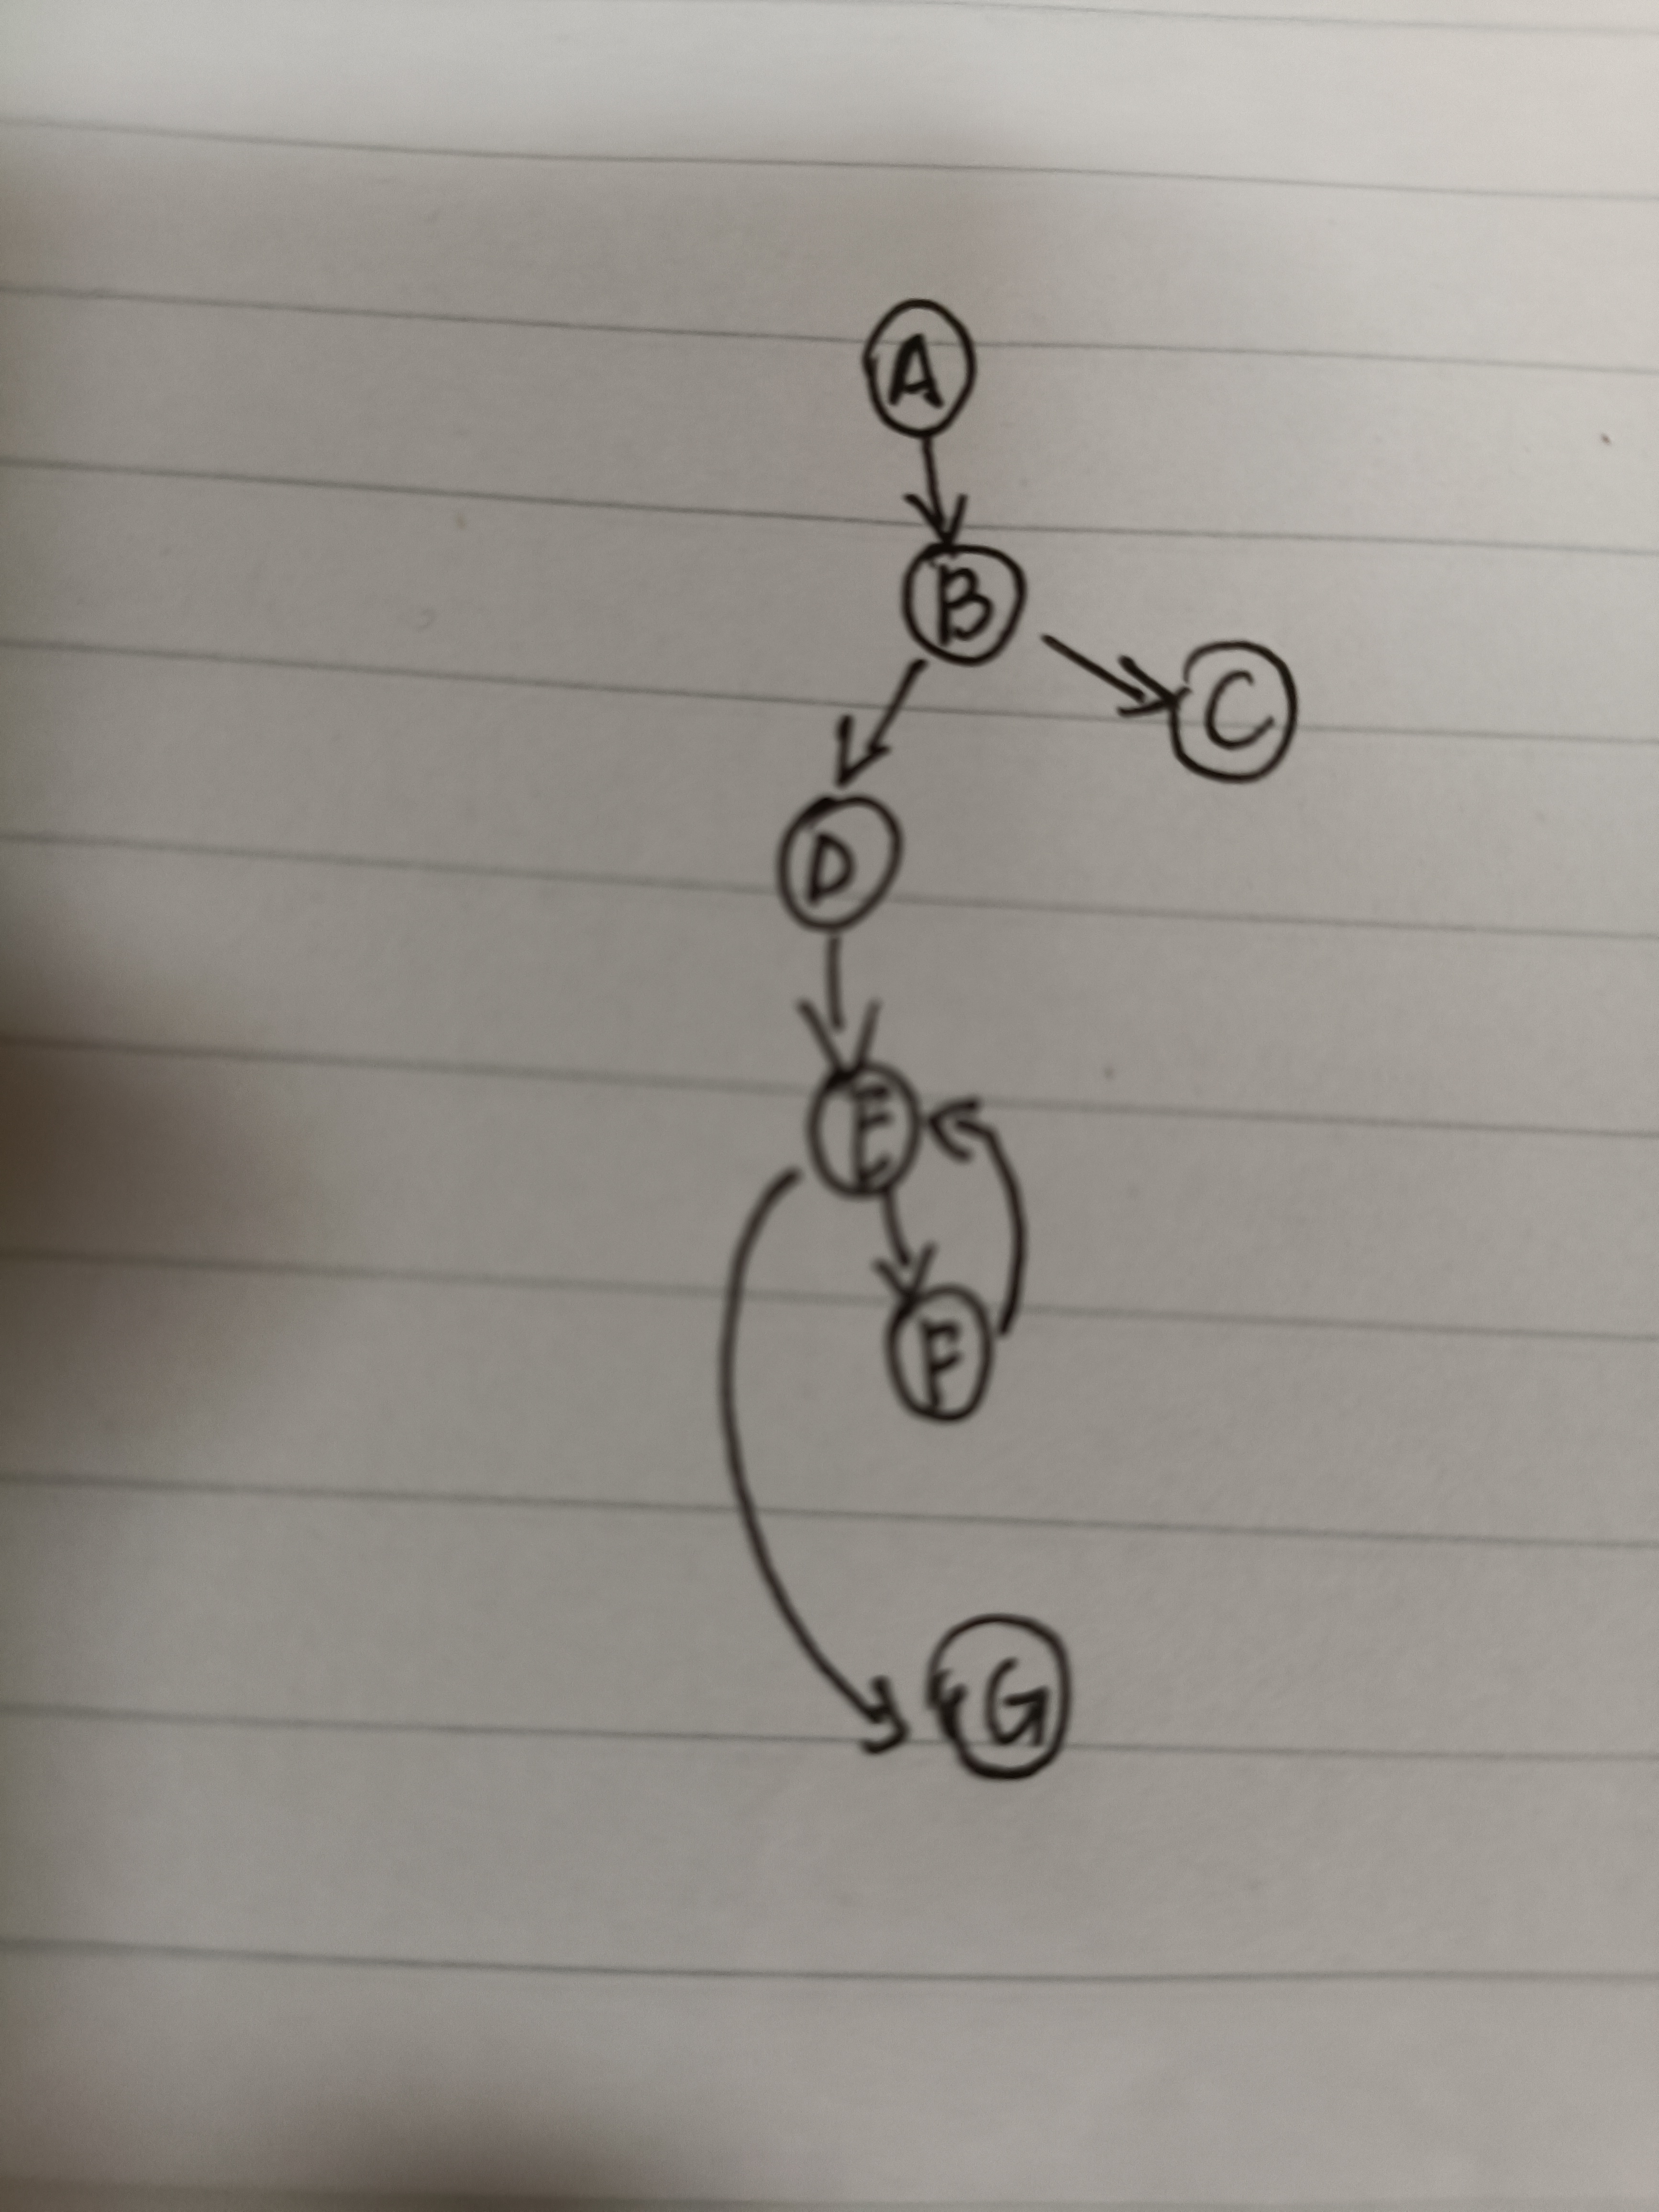
\includegraphics[scale=0.06]{screenshots/DD-minimum.jpg}

数据流分析如下

\begin{table}[!h]
    \begin{tabular}{|l|l|l|}
    \hline
    变量名 & 定义节点 & 使用节点 \\ \hline
    this.mRoot & A & B D\\ \hline
    p & D & E F G \\ \hline
    \end{tabular}
\end{table}

在这个方法的单元测试中,使用数据流分析的结果设计用例,覆盖指标采用\textbf{全使用准则}。
因此,测试用例的执行路径集合,需要覆盖以下路径:A-B, A-D, D-E, D-F, D-G.

\subsection{用例设计}

在红黑树为空的时候,查询一次maximum。然后构建一棵与search方法单元测试中相同的红黑树,再查询一次maximum。具体可见代码实现。

\section{对leftRotate方法的测试}

leftRotate方法代码如下

\begin{lstlisting} [language = Java]
public void leftRotate(RBTNode<T> x) {
    // 设置x的右孩子为y
    RBTNode<T> y = x.right;

    // 将 “y的左孩子” 设为 “x的右孩子”;
    // 如果y的左孩子非空,将 “x” 设为 “y的左孩子的父亲”
    x.right = y.left;
    if (y.left != null)
        y.left.parent = x;

    // 将 “x的父亲” 设为 “y的父亲”
    y.parent = x.parent;

    if (x.parent == null) {
        this.mRoot = y;            // 如果 “x的父亲” 是空节点,则将y设为根节点
    } else {
        if (x.parent.left == x)
            x.parent.left = y;    // 如果 x是它父节点的左孩子,则将y设为“x的父节点的左孩子”
        else
            x.parent.right = y;    // 如果 x是它父节点的左孩子,则将y设为“x的父节点的左孩子”
    }
    
    // 将 “x” 设为 “y的左孩子”
    y.left = x;
    // 将 “x的父节点” 设为 “y”
    x.parent = y;
}
\end{lstlisting}

\subsection{DD路径分析和数据流分析}

各个节点的定义如下

\begin{table}[!h]
    \begin{tabular}{|l|l|}
    \hline
    代码行 & DD路径名称\\ \hline
    1-7 & A\\ \hline
    8 & B\\ \hline
    9 & C \\ \hline
    12 & D \\ \hline
    14 & E \\ \hline
    15 & F \\ \hline
    17 & G \\ \hline
    18 & H \\ \hline
    19-20 & I \\ \hline
    23-26 & J \\ \hline
    \end{tabular}
\end{table}

DD路径如下

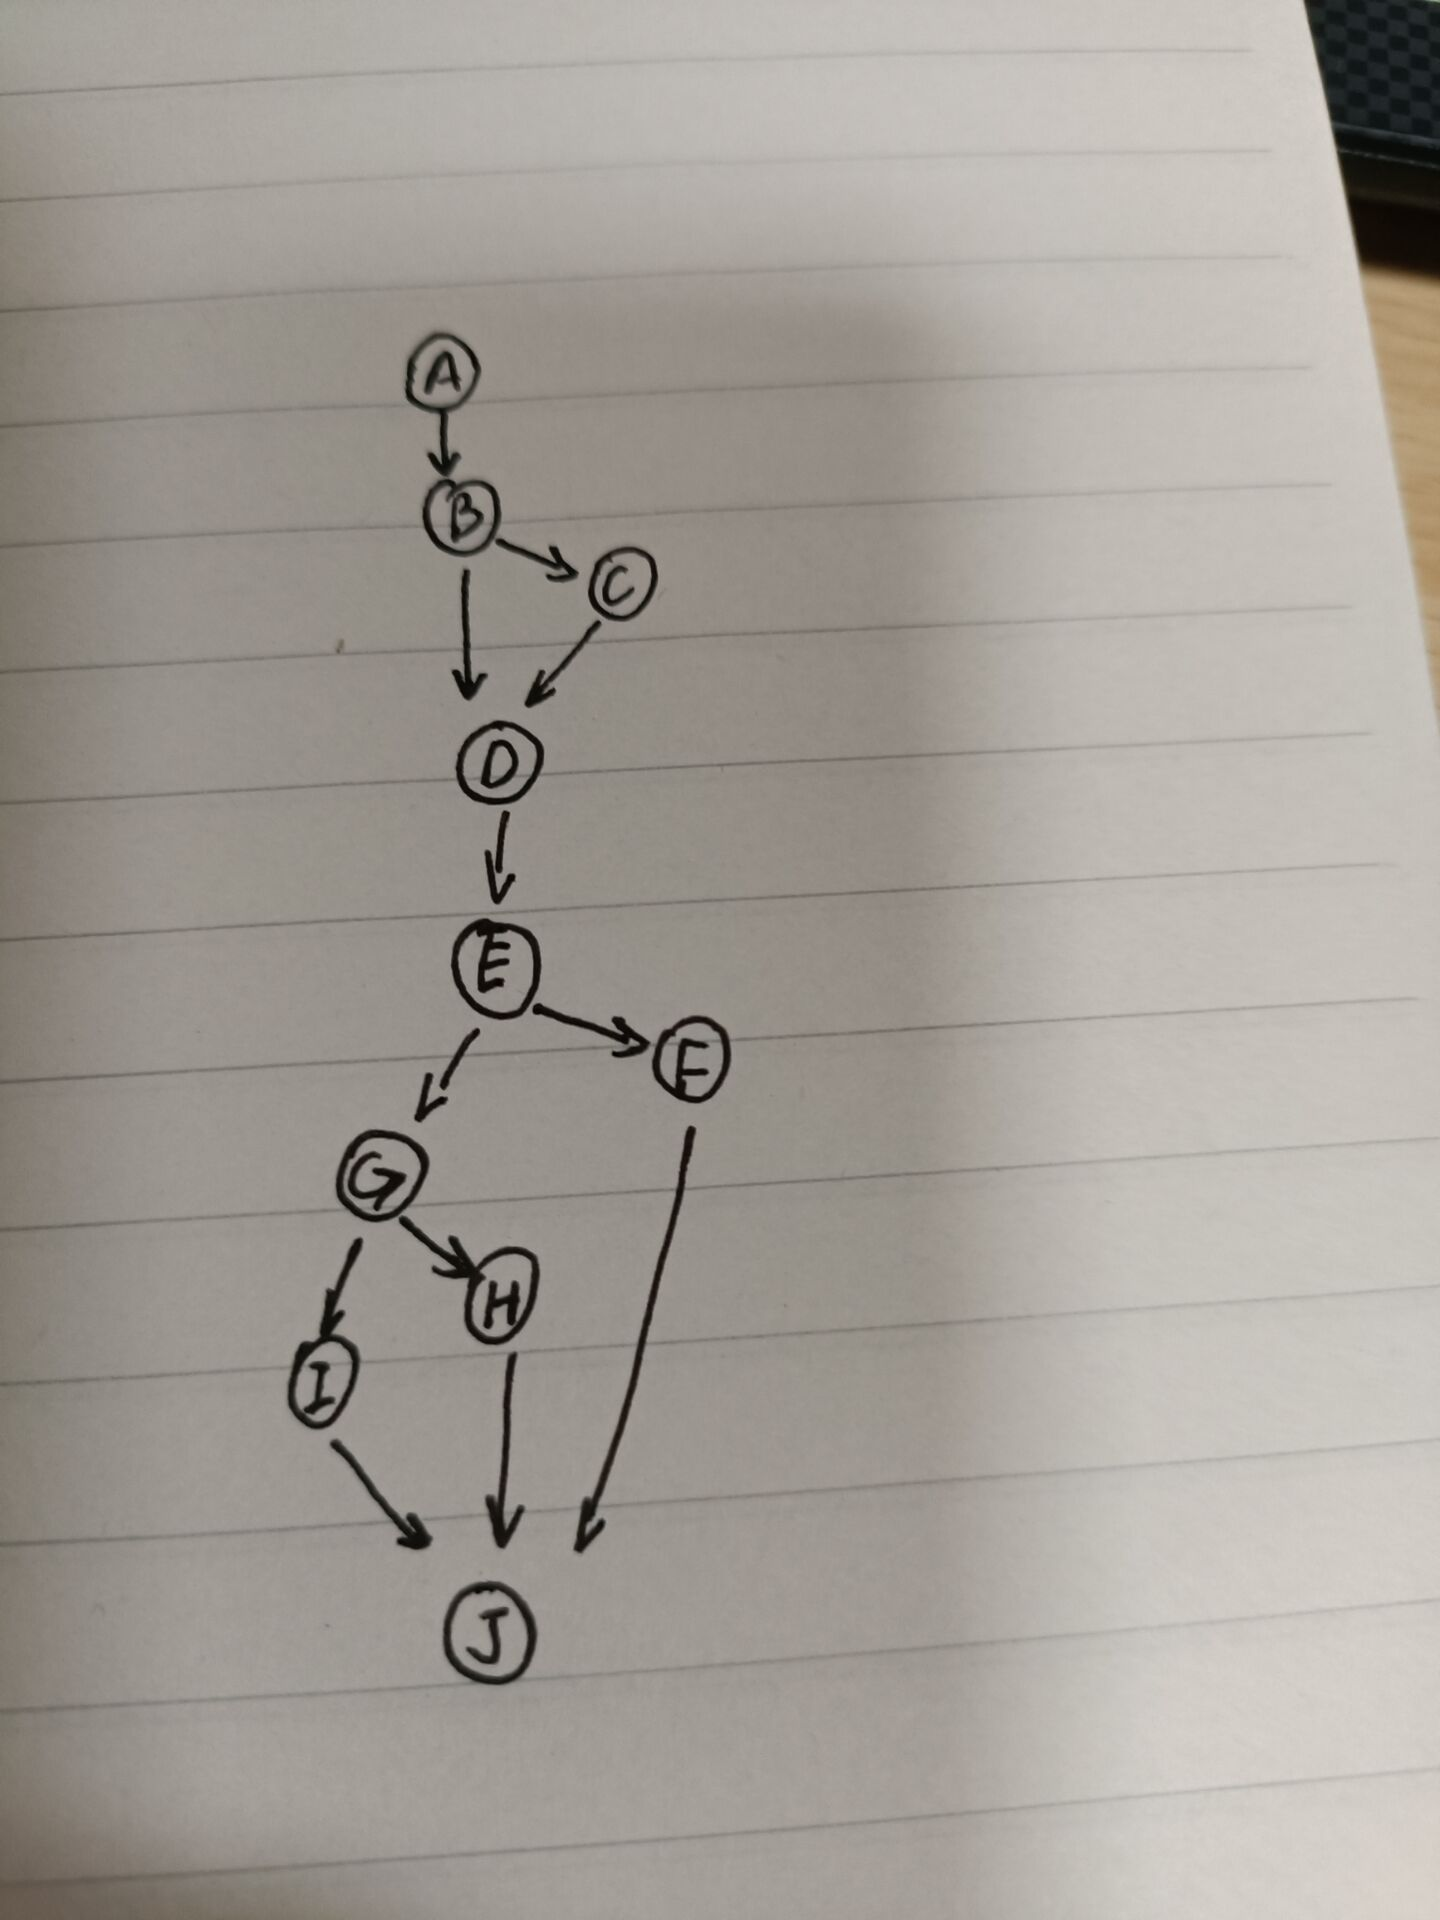
\includegraphics[scale=0.2]{screenshots/DD-leftRotate.jpg}

数据流分析如下

\begin{table}[!h]
    \begin{tabular}{|l|l|l|}
    \hline
    变量名 & 定义节点 & 使用节点 \\ \hline
    x & A & A C D E G H I J\\ \hline
    y & A & A B C D F H I J \\ \hline
    this.mRoot & A & F \\ \hline
    \end{tabular}
\end{table}

在这个方法的单元测试中,使用DD-路径分析的结果设计用例,覆盖指标采用$C_1p$。
因此,可以设计恰当的用例,使得控制流分别如下经过以下三个路径

A B C D E F J

A B D E G H J

A B D E G I J

\subsection{用例设计}

先构造一棵红黑树,分别旋转三个节点使得控制流满足上述的三个路径。具体做法可见代码以及代码内注释。

\section{对rightRotate方法的测试}

rightRotate方法与leftRotate方法有对称性。代码如下

\begin{lstlisting} [language = Java]
public void rightRotate(RBTNode<T> y) {
    // 设置x是当前节点的左孩子。
    RBTNode<T> x = y.left;

    // 将 “x的右孩子” 设为 “y的左孩子”;
    // 如果"x的右孩子"不为空的话,将 “y” 设为 “x的右孩子的父亲”
    y.left = x.right;
    if (x.right != null)
        x.right.parent = y;

    // 将 “y的父亲” 设为 “x的父亲”
    x.parent = y.parent;

    if (y.parent == null) {
        this.mRoot = x;            // 如果 “y的父亲” 是空节点,则将x设为根节点
    } else {
        if (y == y.parent.right)
            y.parent.right = x;    // 如果 y是它父节点的右孩子,则将x设为“y的父节点的右孩子”
        else
            y.parent.left = x;    // (y是它父节点的左孩子) 将x设为“x的父节点的左孩子”
    }

    // 将 “y” 设为 “x的右孩子”
    x.right = y;

    // 将 “y的父节点” 设为 “x”
    y.parent = x;
}
\end{lstlisting}

\subsection{DD路径分析和数据流分析}

各个节点的定义如下

\begin{table}[!h]
    \begin{tabular}{|l|l|}
    \hline
    代码行 & DD路径名称\\ \hline
    1-7 & A\\ \hline
    8 & B\\ \hline
    9 & C \\ \hline
    12 & D \\ \hline
    14 & E \\ \hline
    15 & F \\ \hline
    17 & G \\ \hline
    18 & H \\ \hline
    19-20 & I \\ \hline
    23-26 & J \\ \hline
    \end{tabular}
\end{table}

DD路径如下

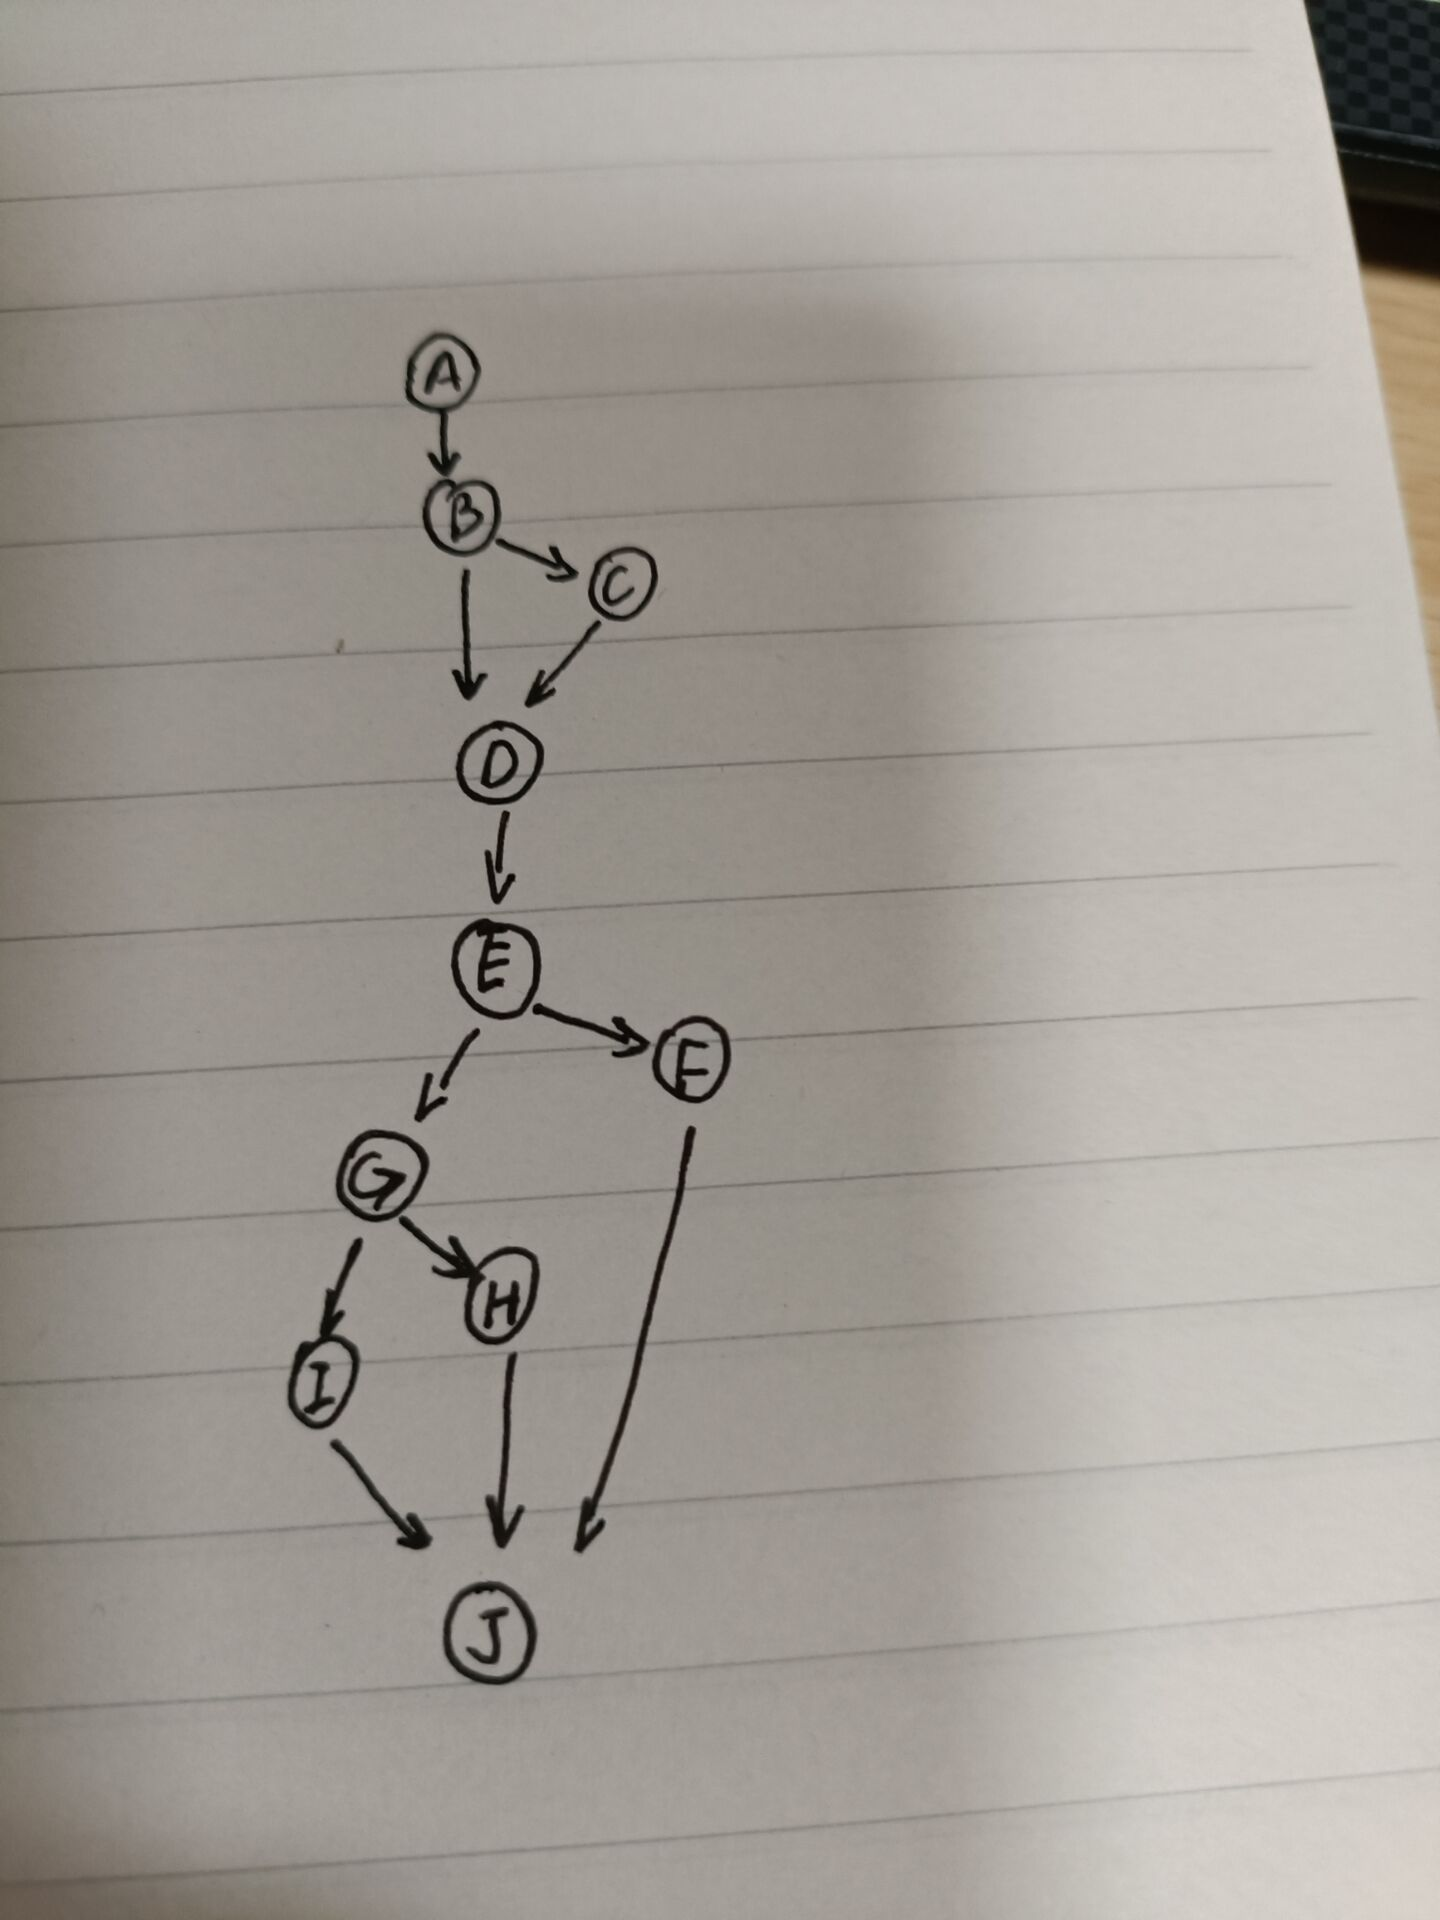
\includegraphics[scale=0.2]{screenshots/DD-leftRotate.jpg}

数据流分析如下

\begin{table}[!h]
    \begin{tabular}{|l|l|l|}
    \hline
    变量名 & 定义节点 & 使用节点 \\ \hline
    y & A & A B C D F H I J \\ \hline
    x & A & A C D E G H I J\\ \hline
    this.mRoot & A & F \\ \hline
    \end{tabular}
\end{table}

在这个方法的单元测试中,使用DD-路径分析的结果设计用例,覆盖指标采用$C_1p$。
因此,可以设计恰当的用例,使得控制流分别如下经过以下三个路径

A B C D E F J

A B D E G H J

A B D E G I J

\subsection{用例设计}

与leftRotate相同,先构造一棵红黑树,分别旋转三个节点使得控制流满足上述的三个路径。具体做法可见代码以及代码内注释。

\end{document}
